\documentclass[journal]{IEEEtran}
\usepackage[english]{babel}

\usepackage{amssymb, amsmath} %Paquetes matemáticos de la American Mathematical 
\usepackage[utf8]{inputenc}
\usepackage{graphicx}
\usepackage{float}
\usepackage{hyperref}
\usepackage{listings}
\usepackage{xcolor}

\definecolor{codegreen}{rgb}{0,0.6,0}
\definecolor{codegray}{rgb}{0.5,0.5,0.5}
\definecolor{codepurple}{rgb}{0.58,0,0.82}
\definecolor{backcolour}{rgb}{0.95,0.95,0.92}
% Definicio de estilo para el codigo fuente que se cita
\lstdefinestyle{mystyle}{
    backgroundcolor=\color{backcolour},   
    commentstyle=\color{codegreen},
    keywordstyle=\color{magenta},
    numberstyle=\tiny\color{codegray},
    stringstyle=\color{codepurple},
    basicstyle=\ttfamily\footnotesize,
    breakatwhitespace=false,         
    breaklines=true,                 
    captionpos=b,                    
    keepspaces=true,
    numbers=left,                    
    numbersep=5pt,                  
    showspaces=false,                
    showstringspaces=false,
    showtabs=false,                  
    tabsize=2,
}
\lstset{style=mystyle}

\renewcommand{\lstlistingname}{Código}

\ifCLASSINFOpdf

\else

\fi

\hyphenation{op-tical net-works semi-conduc-tor}


\begin{document}

\title{Ejercicio 1 - tema 2 \\ Juegos de caracteres y componentes de la BD.}
%
\author{Vicente Romero Andrade}

\markboth{Ejercicio 1 - tema 2 Juegos de caracteres y componentes de la BD., Marzo~2021}%
{Shell \MakeLowercase{\textit{et al.}}: }
% The only time the second header will appear is for the odd numbered pages

\maketitle


\IEEEpeerreviewmaketitle

\section{Objetivo}
% The very first letter is a 2 line initial drop letter followed

\IEEEPARstart{E}{l} objetivo es, comprender la importancia de los juegos de caracteres durante el proceso de instalación de una base de datos, conocer la forma en la que se 
pueden consultar los diferentes componentes instalados en una base de datos y calcular el espacio en disco que ocupan.


\section{Desarrollo}
\subsection{C1. Juego de caracteres}
\subsubsection{¿Qué significa AL32UTF8?}
Significa "All Language 32 Unicode Transformation Format".
\subsubsection{¿Cuál es la longitud máxima que puede tener un carácter con esta configuración?}
4 bytes.
\subsubsection{¿En qué casos un carácter requeriría la longitud máxima para poder almacenarse?}
Cuando se usen los caracteres suplementarios que se encuentran definidos en las últimas versiones
del estándar Unicode.
\subsubsection{¿Por qué Oracle recomienda este juego de caracteres?}
Porque UTF8 ya no recibe nuevas versiones del estándar Unicode y AL32UTF8 si, por lo que este último
soporta mayor cantidad de caracteres.
\subsubsection{¿Qué desventajas y en qué situaciones no se recomendaría este valor?}
Cuando se requiera una compatibilidad estricta con aplicaciones externas a la base de datos de Oracle.
\subsection{C2. Codigo del script}
\lstinputlisting[language=sql,caption=s-01-database-info.sql,label={lst:scriptsql}]{s-01-database-info.sql}
\subsection{C3. Salida de ejecución del script anterior}
\begin{figure}[H]
  \centering
  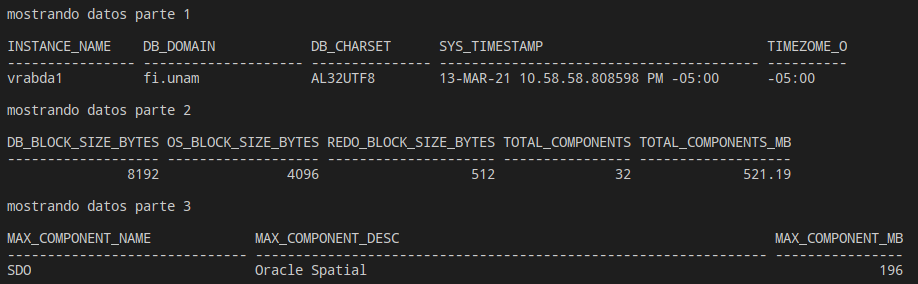
\includegraphics[scale=.27]{salida_ej1_t2.png}
   \caption{Salida del script}
   \label{fig:salidascript}
\end{figure}
\subsection{C4. Salida de ejecución del validador}
\begin{figure}[H]
  \centering
  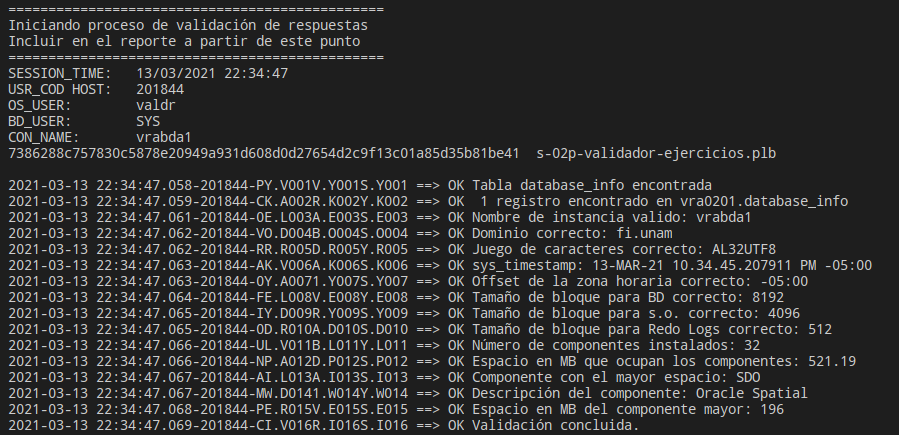
\includegraphics[scale=.27]{validador_ej1_t2.png}
   \caption{Salida del validador}
   \label{fig:validador}
\end{figure}
\section{Conclusiones}
En este ejercicio se vieron los componentes de la base de datos que 
son necesarios conocer antes de poder crear una nueva base, estos
son importantes conocerlos para poder hacer estimaciones de los 
recursos que van a ser necesarios más adelante. La única dificultad
fue hacer que coincidiera el timezone\_offset con el del validador,
podría añadirse una sección para cambiar la zona horaria de la base de datos.
\ifCLASSOPTIONcaptionsoff
  \newpage

\fi

\begin{thebibliography}{2}
  \bibitem{oracle_white}
  "An Oracle White Paper", 
  Oracle.com, 2005. [Online]. 
  Available: http://www.oracle.com/technetwork/products/globalization/twp-appdev-unicode-10gr2-129234.pdf. 
  [Accessed: 13- Mar- 2021].
\end{thebibliography}
\end{document}
